\documentclass[12pt]{article}
\RequirePackage{amsthm,amsmath,amsbsy,amsfonts}
\usepackage{graphicx}
%\usepackage{enumerate}
\usepackage{natbib}
\usepackage{url} % not crucial - just used below for the URL 
\usepackage{placeins}

%\pdfminorversion=4
% NOTE: To produce blinded version, replace "0" with "1" below.
\newcommand{\blind}{0}

% DON'T change margins - should be 1 inch all around.
\addtolength{\oddsidemargin}{-.5in}%
\addtolength{\evensidemargin}{-.5in}%
\addtolength{\textwidth}{1in}%
\addtolength{\textheight}{1.3in}%
\addtolength{\topmargin}{-.8in}%


\begin{document}
	\title{Supplementary Material}	 
	\begin{figure}[h!]
		\caption{F1 score by threshold, data size, and method (1 is best 0 is worst).}
		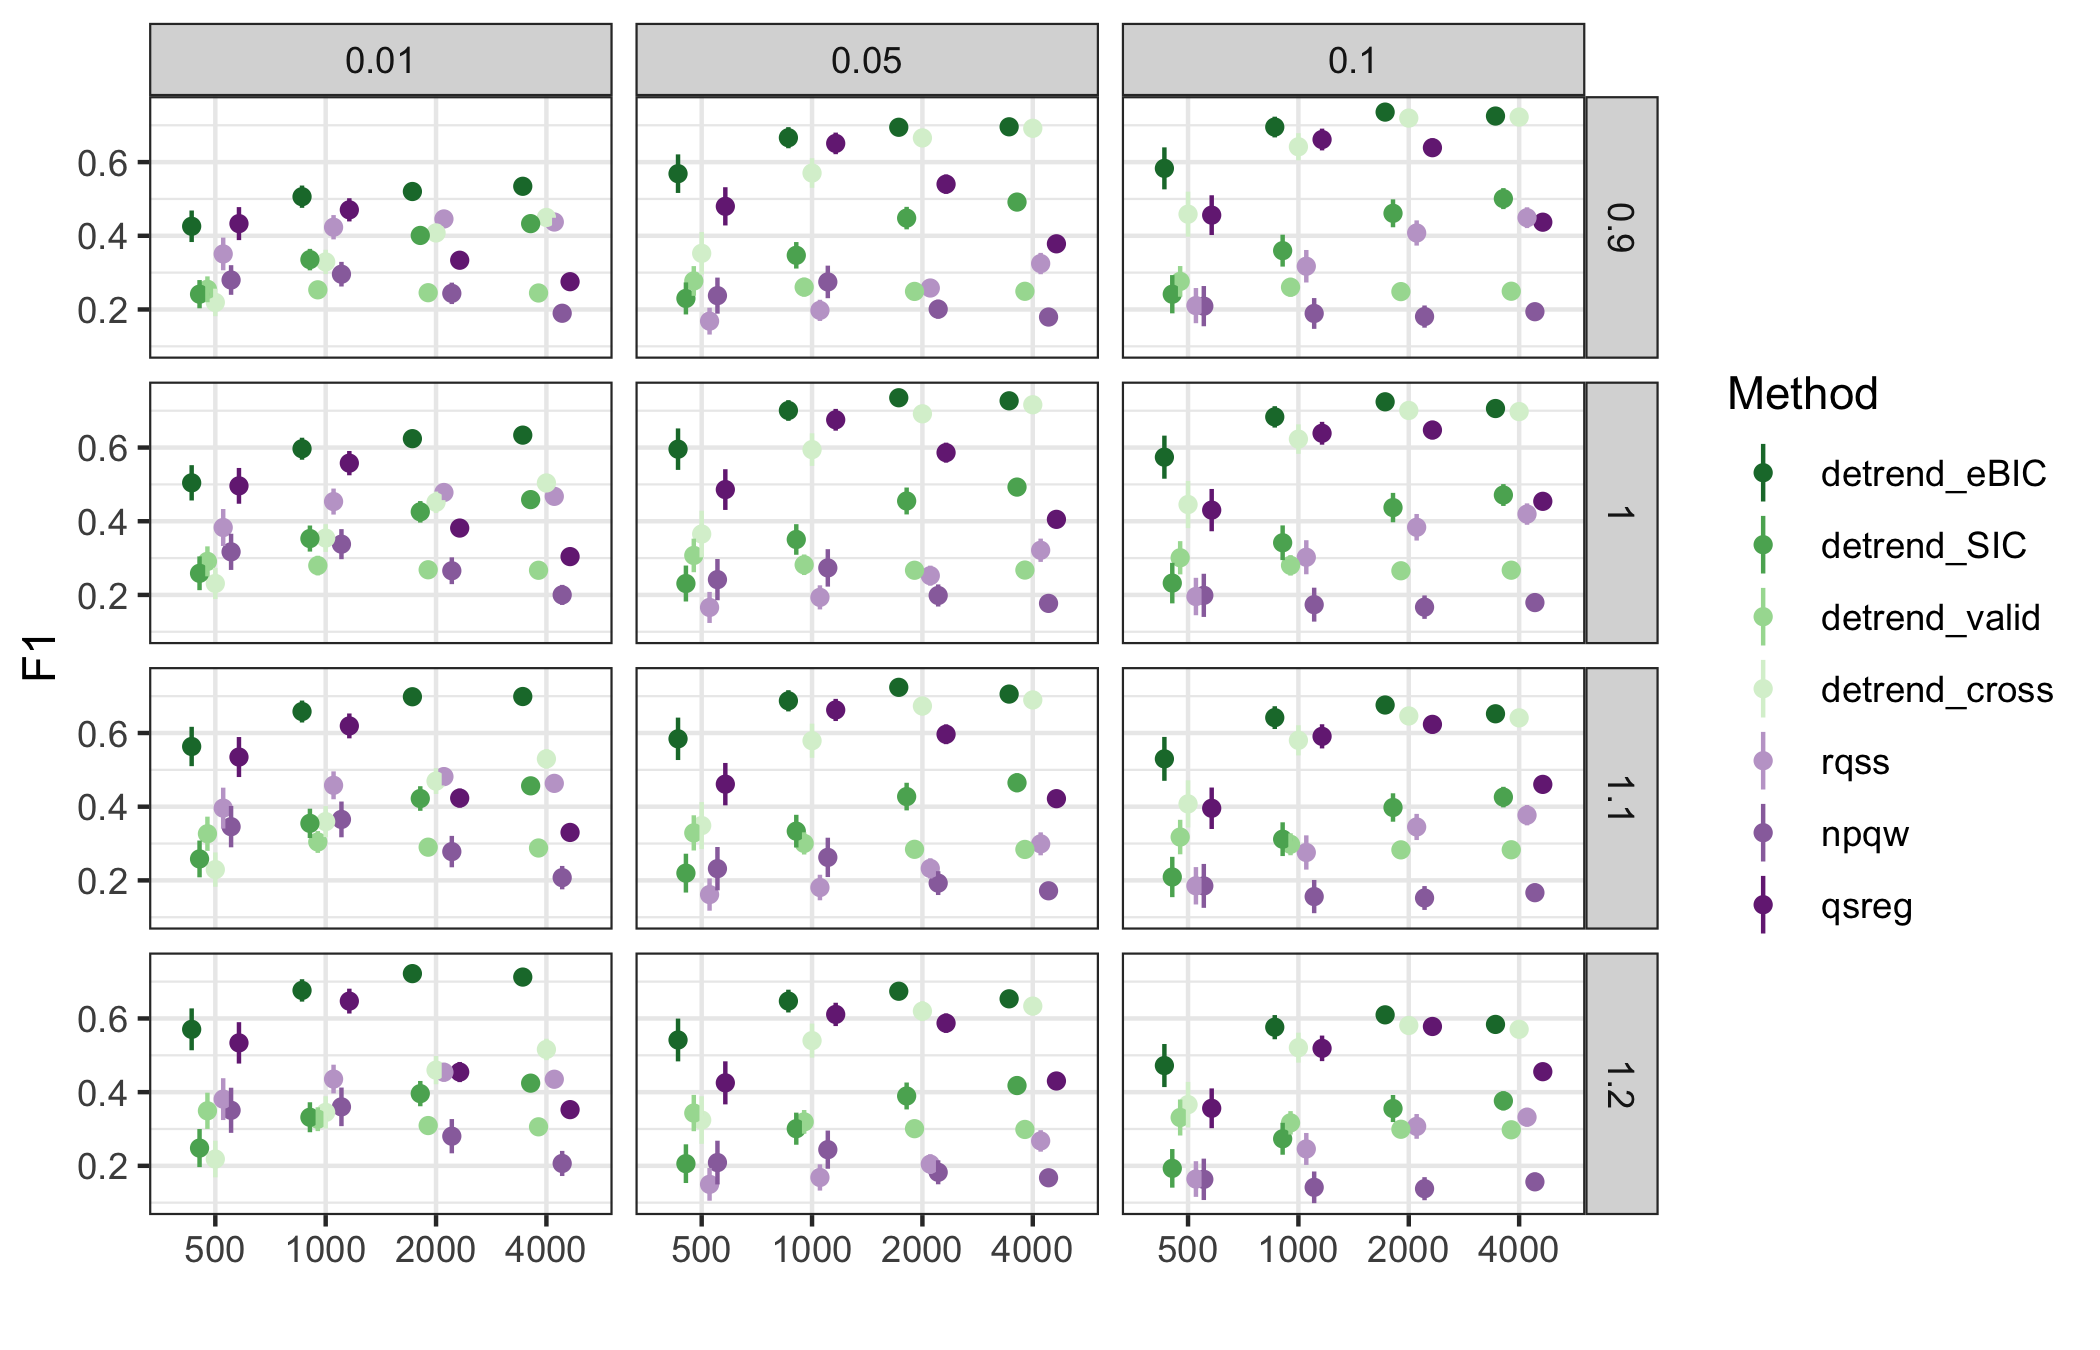
\includegraphics[width = \linewidth]{Figures/peaks_F1.png}
	\end{figure}
	
	\begin{figure}[h!]
		\caption{Precision by threshold, data size, and method (true positive over true positives + false positives).}
		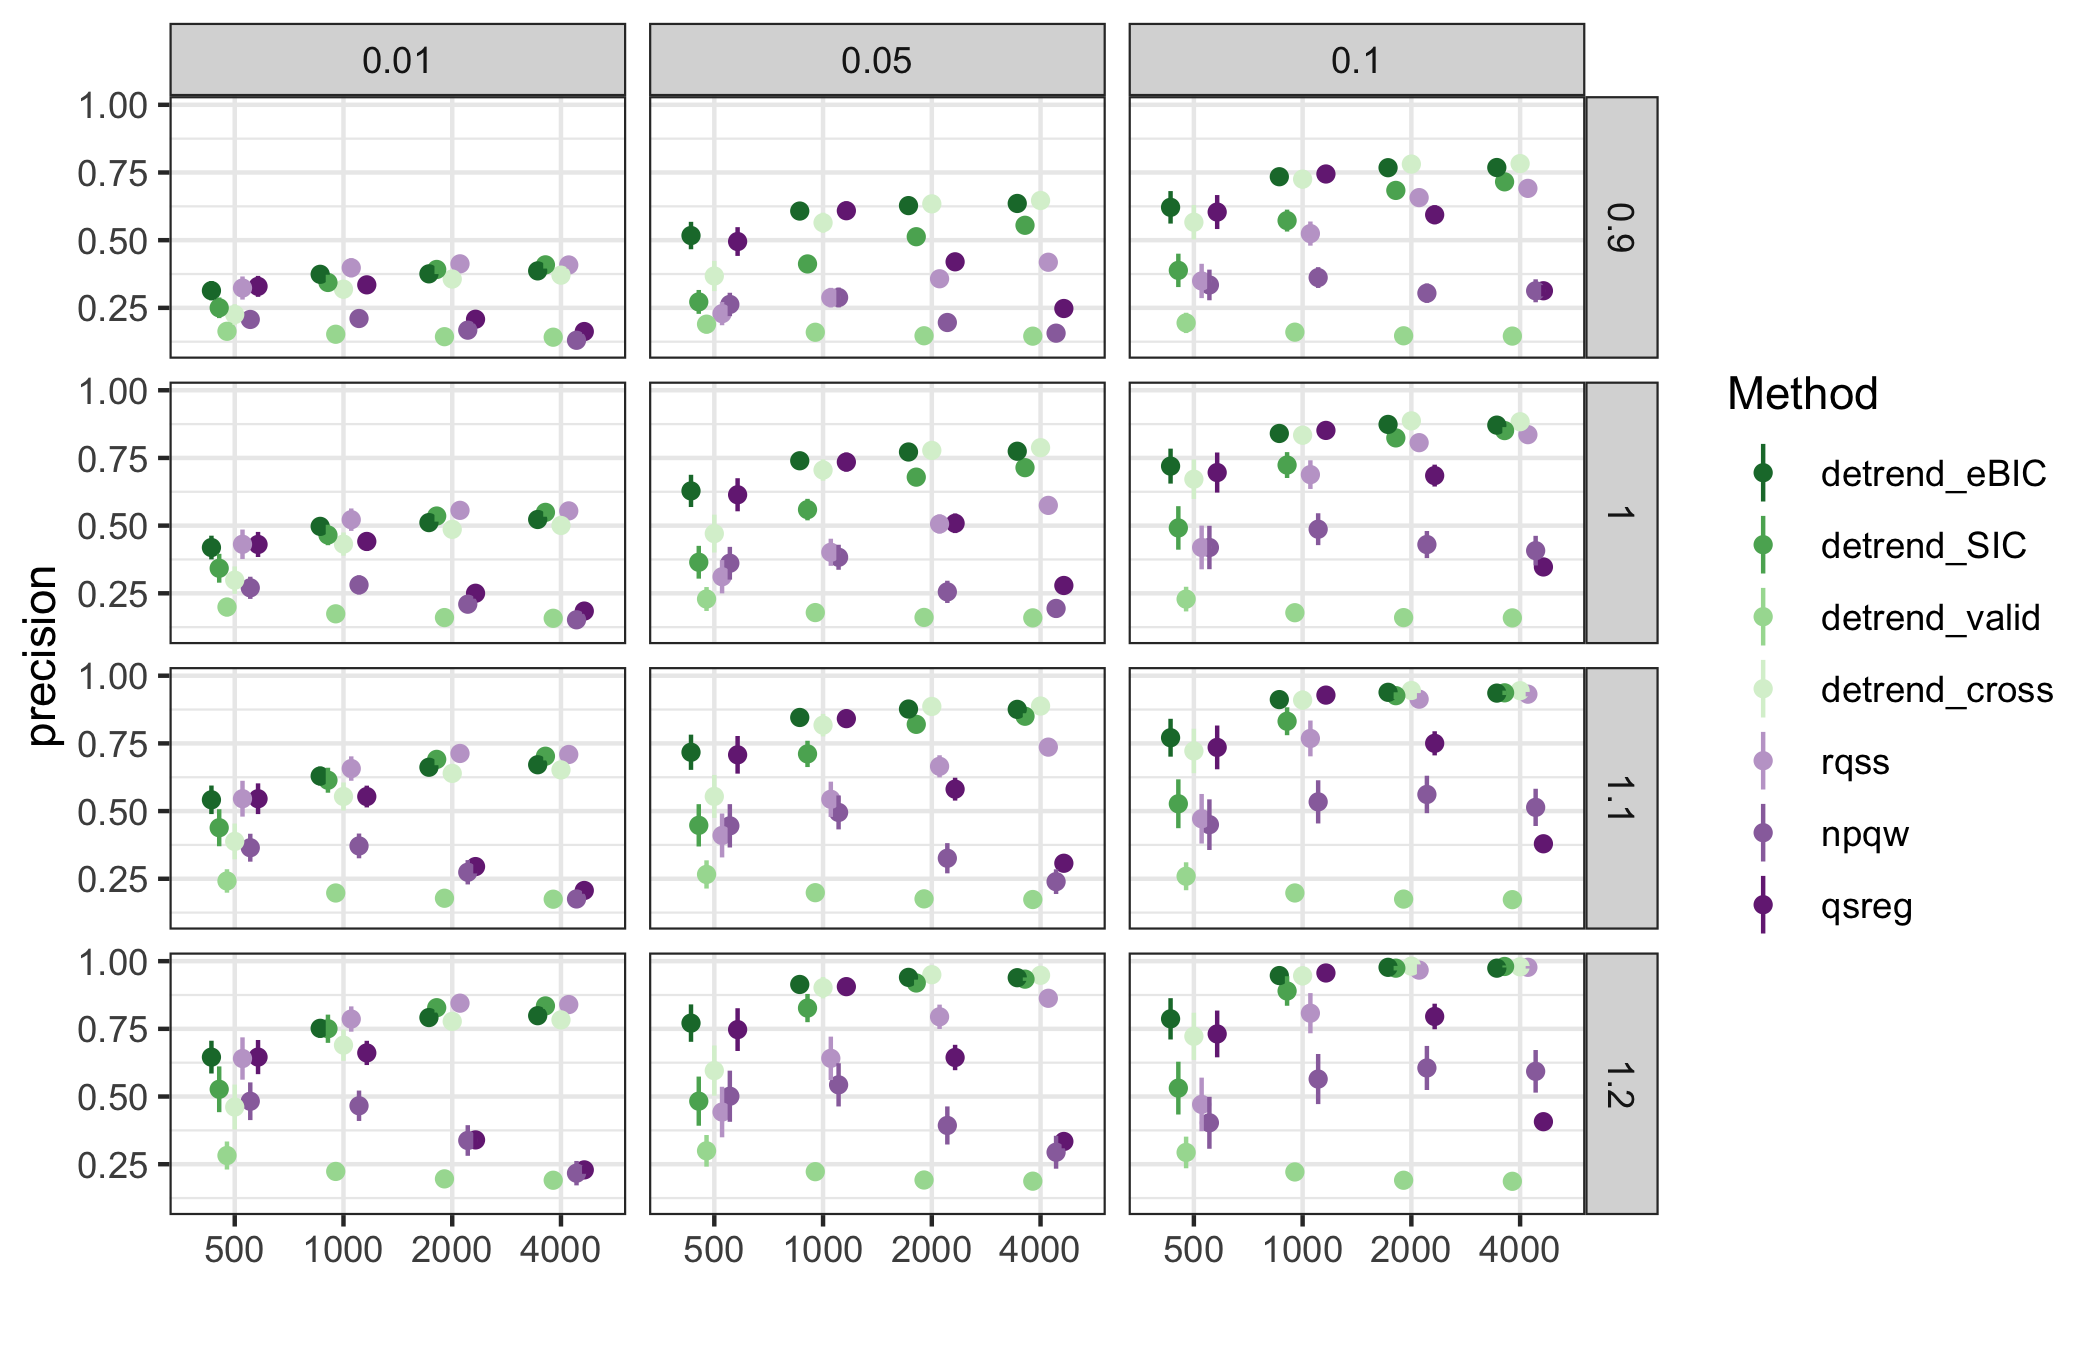
\includegraphics[width = \linewidth]{Figures/peaks_precision.png}
	\end{figure}
	
	\begin{figure}[h!]
		\caption{Recall by threshold, data size, and method (true positive over true positives + false negatives).}
		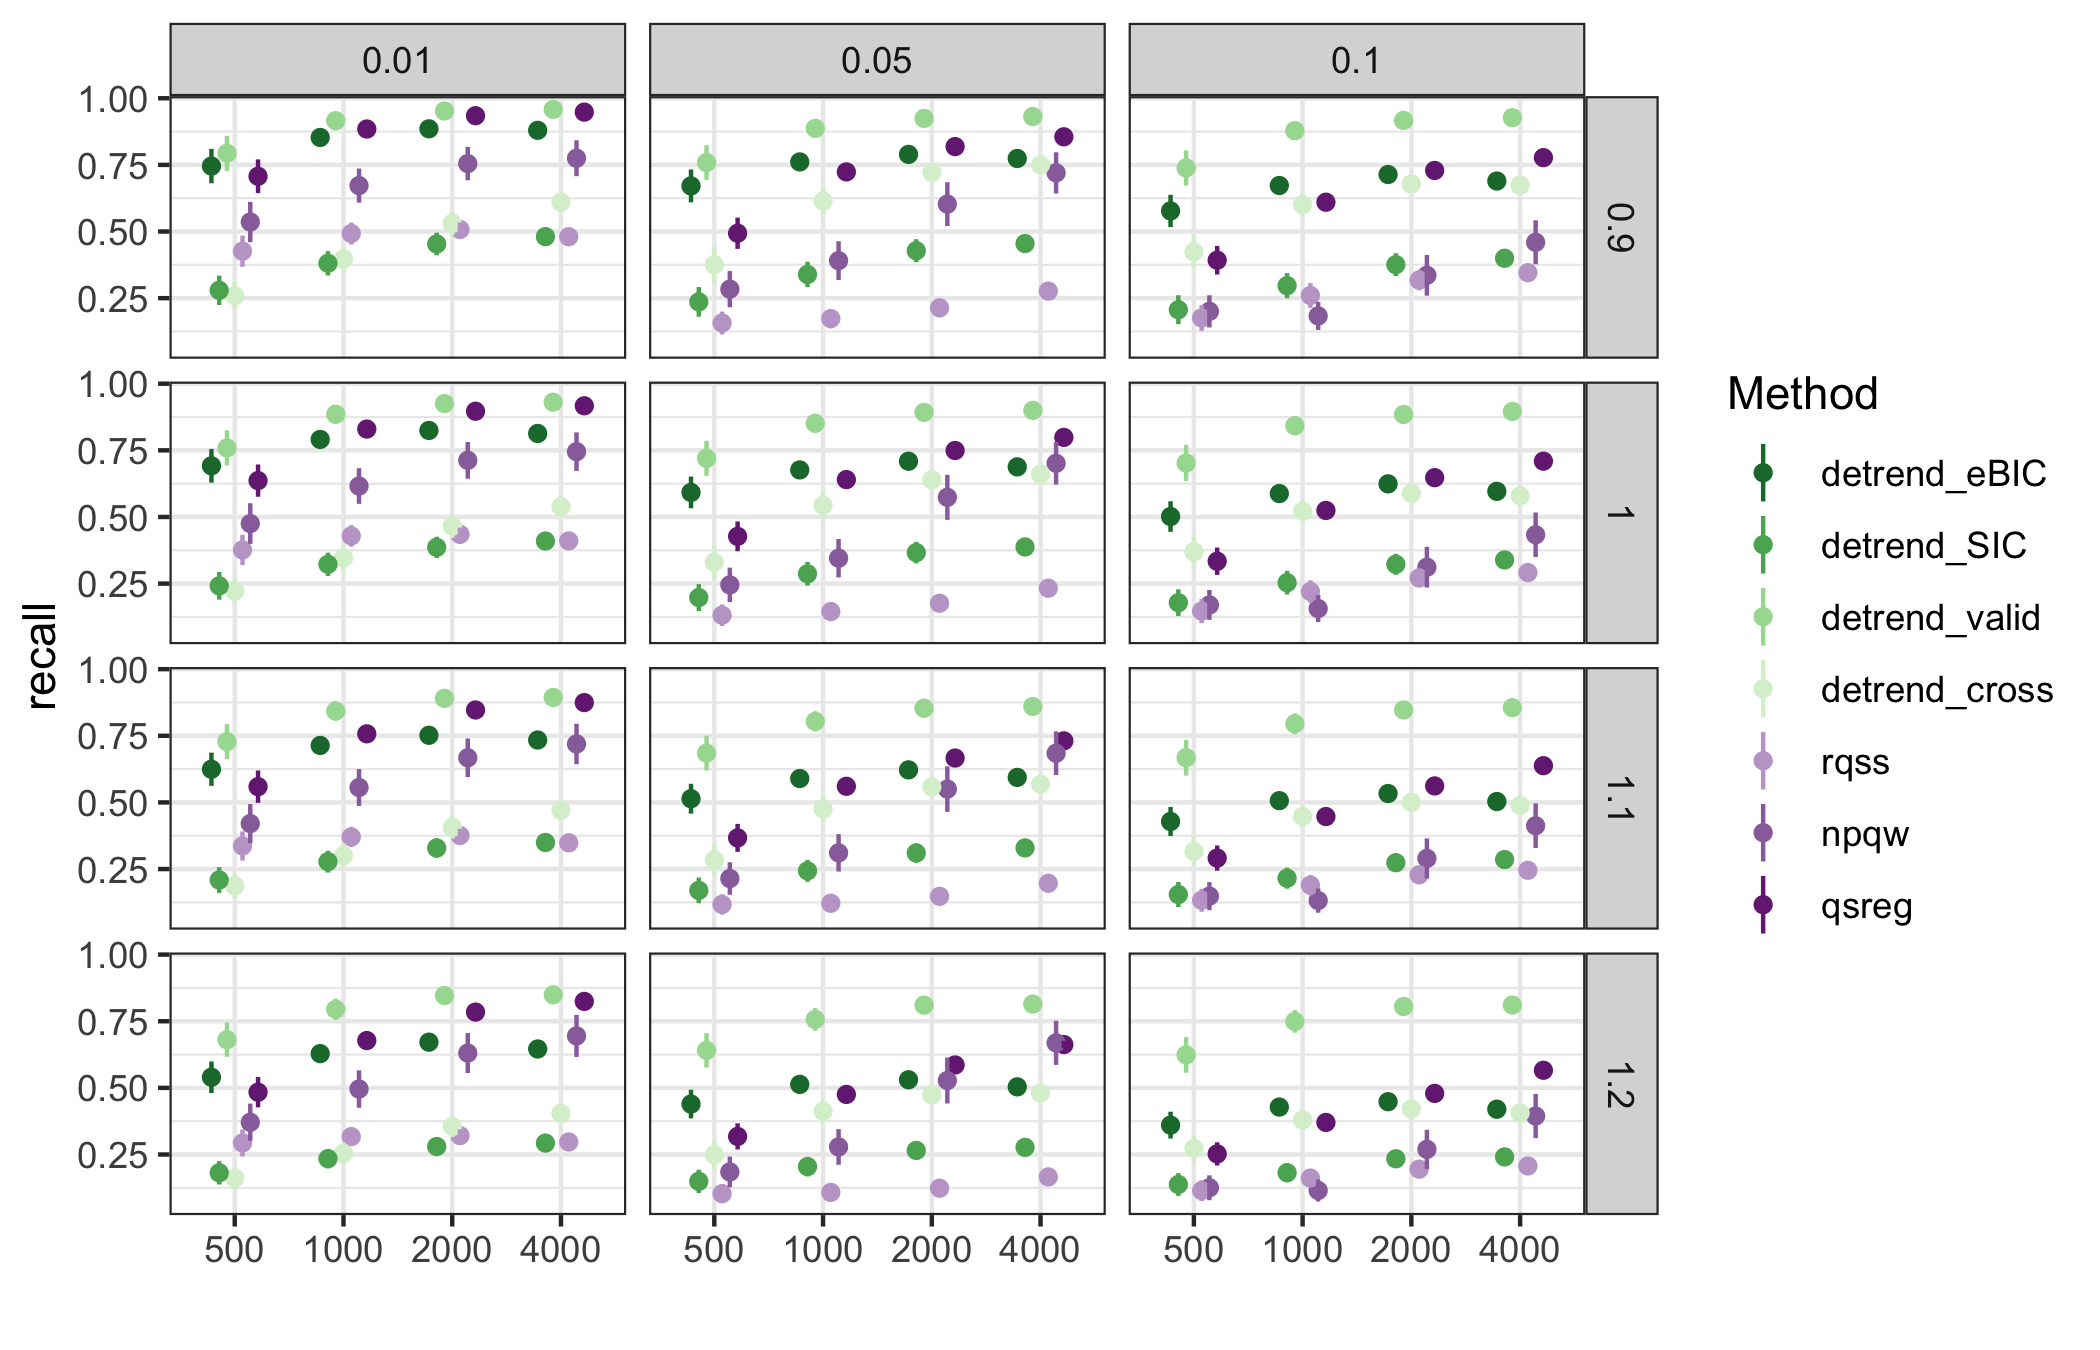
\includegraphics[width = \linewidth]{Figures/peaks_recall.png}
	\end{figure}
	
	\begin{figure}[h!]
		\caption{Miss-classification rates by threshold, data size, and method, values above the upper limit (npqw) not shown.}
		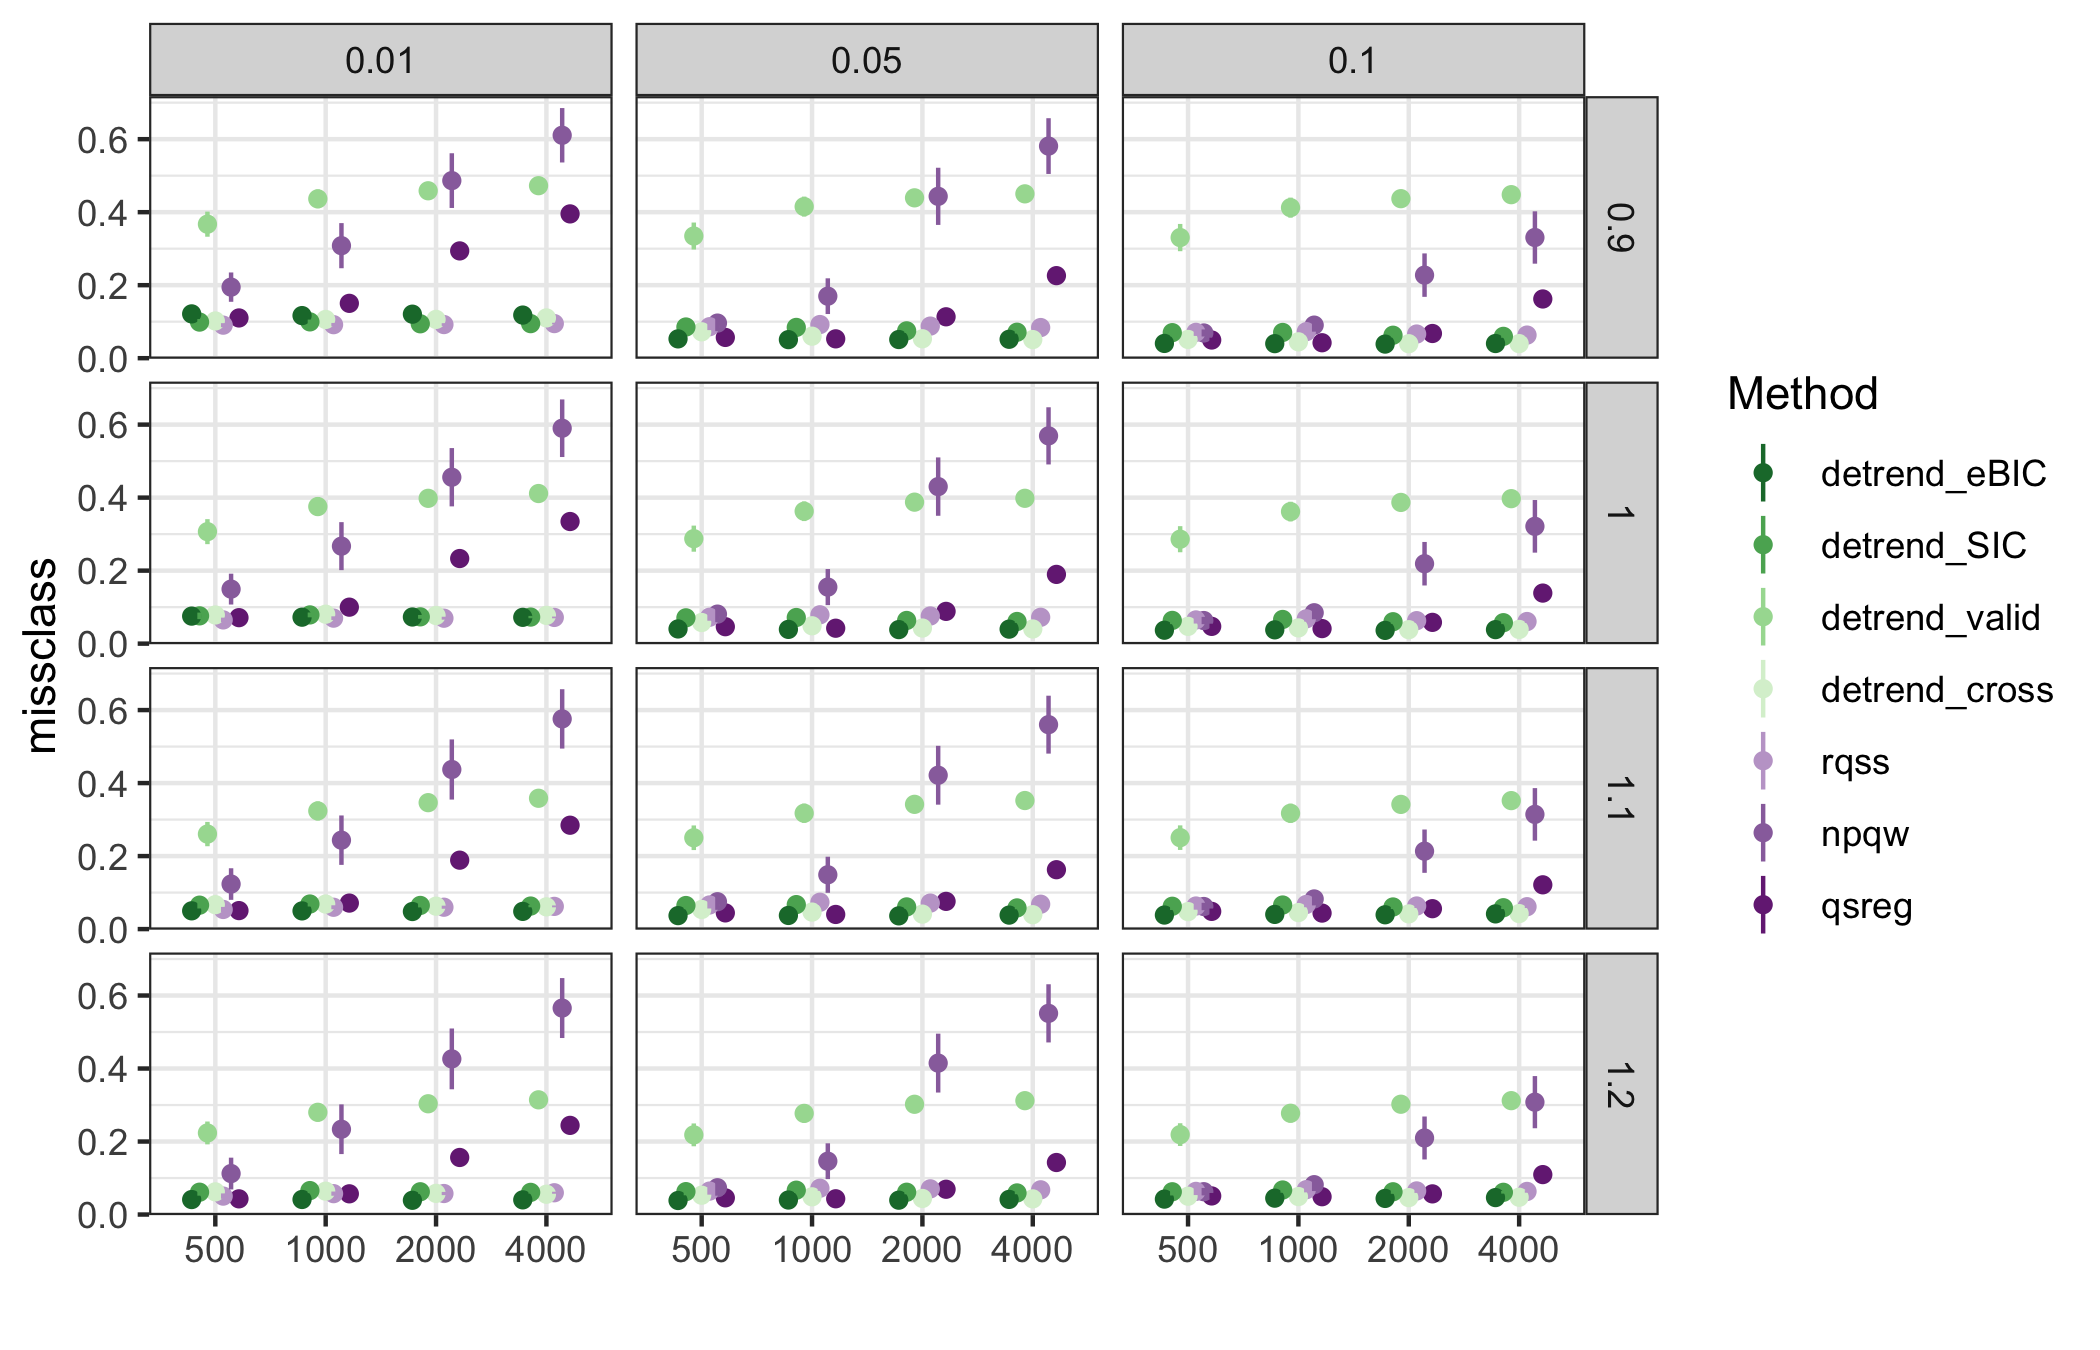
\includegraphics[width = \linewidth]{Figures/peaks_missclass.png}
	\end{figure}

\end{document}